\chapter{Implementation}

In this chapter, we put forth our research and implementation. First, present
the analysis of previous work regarding gas consumption, cost in fiat and
security. Then we gradually describe our improved methodology that eliminates
storage by utilizing hash-and-resubmit technique and delivers a gas-efficient,
superlight Bitcoin client implementation. \todo{extend intro}

\section{Analysis of Previous Work}

In this section, we analyse the verifier by Christoglou et. al. First we
discuss the process needed to prepare the code for our analysis. Then, we show
the gas usage of all internal functions of the verifier, and the cost of using
that implementation. Finally, we present the vulnerabilities we discovered, and
how we mitigated them in our work.

\subsection{Porting from old Solidity version}

We used the latest version of Solidity compiler for our analysis. In order to
perform this analysis, we needed to port the verifier from version Solidity 0.4
to version 0.6. The changes we needed to perform were mostly syntactic. These
includes the usage of \texttt{abi.encodePacked}, explicit \texttt{memory} and
\texttt{storage} declaration and explicit cast from \texttt{address} to
\texttt{payable address}. We also used our configured EVMs with EIP 2028(ref)
enabled to benefit from low cost function calls. The functionality of the
contract remained equivalent.

\todo{
The prover’s output is a Proof of Proof of Work that satisfies the above
security parameters. The prover needed to be enhanced in order to create
special test cases (Section(ref)) and enable our optimized architecture
(Section(ref)).
}

\subsection{Gas analysis}

Our profiler measures gas usage per line of code. This is very helpful to
observe detailed gas consumption of a contract. Also, we used Solidity events
to measure aggregated gas consumption of different high-level functionalities
by utilizing the build-in \texttt{gasleft()} function. For our experiment, we
used a chain of 75 blocks and a forked chain at index 55 that spans 10
additional blocks as displayed in Figure \ref{figure:proofs_65-10+20}. Detailed
gas usage of the functionalities of the verifier is shown in Table
\ref{table:old_gas_usage}.

\begin{figure}[hbt]
    \centering
    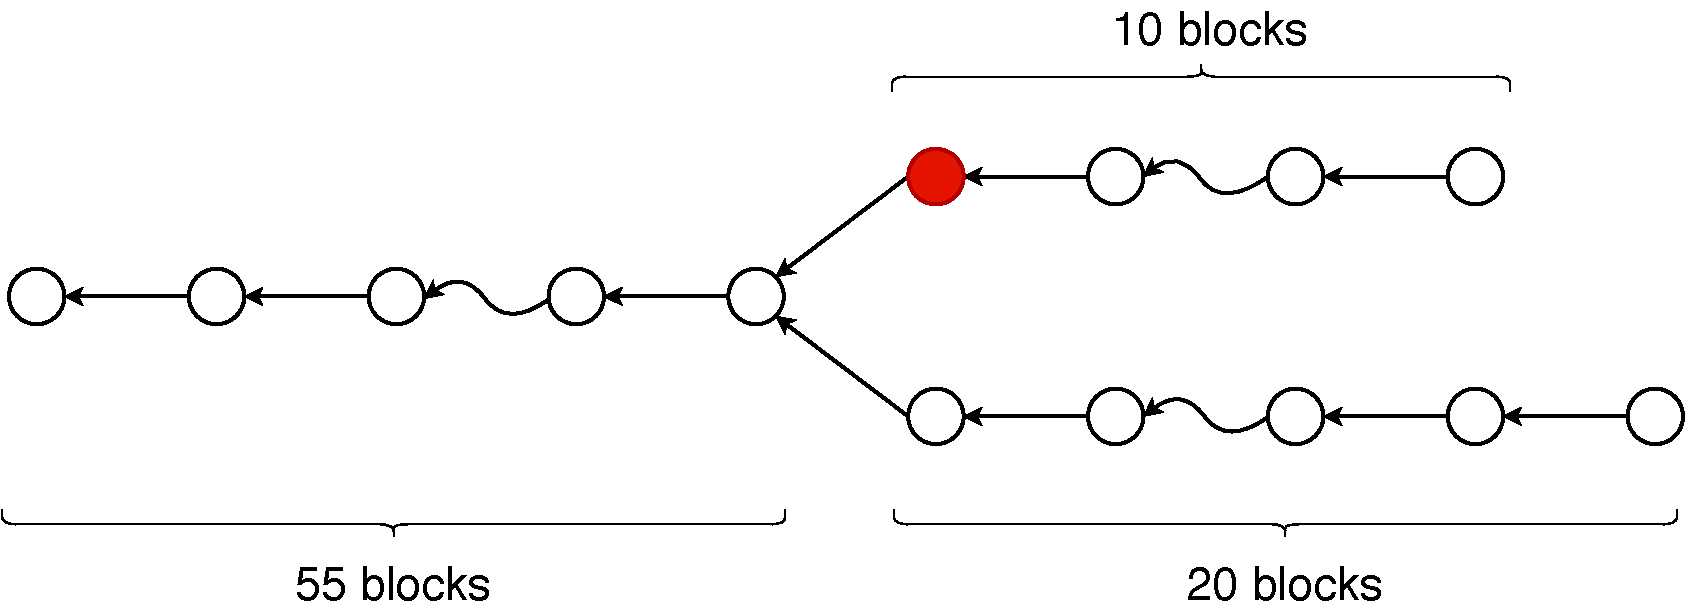
\includegraphics[width=10cm]{./images/proofs_65-10+20.pdf}
    \caption{The red block indicates the block of interest. Curved connections
        imply intermediate blocks. The adversary creates a proof for an event
        that does not exist in the honest chain}
    \label{figure:proofs_65-10+20}
\end{figure}

\begin{table}[H]
    \centering
    \begin{tabular}{@{}lccll@{}}
        \toprule
        \multicolumn{1}{c}{\textbf{Submit function}} & \textbf{gas usage}    \\ \midrule
        validate Interlink  & \multicolumn{1}{r}{   465,604} \\
        \\
        \\
        store proof         & \multicolumn{1}{r}{ 1,044,705} \\
        store DAG           & \multicolumn{1}{r}{ 3,168,612} \\
        store ancestors     & \multicolumn{1}{r}{ 4,995,289} \\
        evaluate predicate  & \multicolumn{1}{r}{   306,433} \\
        delete ancestors    & \multicolumn{1}{r}{    45,137} \\
        \midrule
        Sum                 & \multicolumn{1}{r}{10,025,780} \\
        \bottomrule
    \end{tabular}
    \quad
    \begin{tabular}{@{}lccll@{}}
        \toprule
        \multicolumn{1}{c}{\textbf{Contest function}} & \textbf{gas usage} \\ \midrule
        validate Interlink  & \multicolumn{1}{r}{   485,751} \\
        find LCA            & \multicolumn{1}{r}{ 1,255,523} \\
        compare proofs      & \multicolumn{1}{r}{   447,130} \\
        store proof         & \multicolumn{1}{r}{   304,845} \\
        update DAG          & \multicolumn{1}{r}{ 1,836,578} \\
        store ancestors     & \multicolumn{1}{r}{ 5,584,173} \\
        evaluate predicate  & \multicolumn{1}{r}{   390,307} \\
        delete ancestors    & \multicolumn{1}{r}{    57,023} \\
        \midrule
        Sum                 & \multicolumn{1}{r}{10,361,330} \\
        \bottomrule
    \end{tabular}
    \caption{Execution for proof of 75 blocks}
    \label{table:old_gas_usage}
\end{table}


In this scenario, the original proof is created by an adversary for an event
that does not exist in the honest chain. The proof is contested by an honest
party. We selected this configuration because it includes both phases
(submit and contest) and provides full code coverage of each phase since all
underlying operations are executed and no early returns occur.

For a chain of 75 blocks, each phase of the contract needed more than 10
million gas units. Although the size of this test chain is only a very small
faction of the size of a realistic chain, the gas usage already exceeds the
limit of Ethereum blockchain, which is slightly below 10 million. In
particular, the submit of a 500,0000-blocks chain demands 47,280,453 gas. In
Figure \ref{figure:old_gas_per_chain_proof}, we show gas consumption for submit
phase for different chain sizes and their corresponding proofs sizes. We
demonstrate results for chains sizes from 100 blocks (corresponding proof size
25) to 500,000 blocks (corresponding to proof size 250).

The linear relation displayed in Figure \ref{figure:old_gas_per_proof} implies
that the gas consumption of the verifier is determined by the size of the
proofs. As shown in Figure \ref{figure:size_of_nipopows} \todo{insert figure
for proof size with relation to the chain in Background}, the size of the
proofs grows logarithmically to the size of the chain, and this is also
reflected to the gas consumption curve.

\begin{figure}[ht]
\centering
\begin{subfigure}[b]{.49\textwidth}
\begin{tikzpicture}
    \begin{axis}[
        scaled y ticks = true,
        scaled x ticks = false,
        grid=major,
        width=\textwidth,
        xlabel={Chain size},
        ylabel={Gas consumption}
        ]
    \addplot table [col sep=comma] {data/old_gas_per_chain.csv};
\end{axis}
\end{tikzpicture}
\centering
\caption{Gas consumption per chain size}
\label{figure:old_gas_per_chain}
\end{subfigure}
\begin{subfigure}[b]{.49\textwidth}
\begin{tikzpicture}
    \begin{axis}[
        scaled y ticks = true,
        scaled x ticks = false,
        grid=major,
        width=\textwidth,
        xlabel={Proof size},
        ylabel={Gas consumption}
        ]
    \addplot table [col sep=comma] {data/old_gas_per_proof.csv};
\end{axis}
\end{tikzpicture}
\centering
\caption{Gas consumption per proof size}
\label{figure:old_gas_per_proof}
\end{subfigure}
\caption{Gas consumption with respect to chain and corresponding proof size}
\label{figure:old_gas_per_chain_proof}
\end{figure}



\begin{wraptable}{h}{6.0cm}
    \centering
    \begin{tabular}{@{}lccll@{}}
        \toprule
        \multicolumn{1}{c}{\textbf{Chain size}} & \textbf{Toll}  \\ \midrule
        \multicolumn{1}{r}{    100} & \multicolumn{1}{r}{ 12.43 \euro{} } \\
        \multicolumn{1}{r}{    500} & \multicolumn{1}{r}{ 16.14 \euro{} } \\
        \multicolumn{1}{r}{  1,000} & \multicolumn{1}{r}{ 23.79 \euro{} } \\
        \multicolumn{1}{r}{ 10,000} & \multicolumn{1}{r}{ 33.47 \euro{} } \\
        \multicolumn{1}{r}{ 50,000} & \multicolumn{1}{r}{ 44.03 \euro{} } \\
        \multicolumn{1}{r}{100,000} & \multicolumn{1}{r}{ 45.65 \euro{} } \\
        \multicolumn{1}{r}{500,000} & \multicolumn{1}{r}{ 49.88 \euro{} } \\
        \bottomrule
    \end{tabular}
    \caption{Tolls for different chain sizes. Gas price is Gwei}
    \label{table:old_cost_in_fiat}
\end{wraptable}


\paragraph{Pricing}

So far, we have shown that the verifier is not applicable to the real
blockchain due to extensive gas usage, exceeding the build-in limitation the
Ethereum blockchain by far. While Ethereum adapts to community demands and
build-in parameters can change, it seem improbable to ever incorporate such a
high block gas limit. However, even in this extreme case, the verifier would
still be impractical due to the high cost of the operations in fiat. We call
this amount \emph{toll}, because it is the cost of using the "bridge" between
two blockchains. We list these tolls in Table \ref{table:old_cost_in_fiat}. For
this price, we used gas price equal to 5 Gwei, which is considered an average
amount to complete transactions. With this gas price, the probability
approximately that the transaction will be included in one of the next 200
blocks is 33\%. Note that average gas price will not be sufficient for
contesting phase, and it has to be performed with higher gas price because of
the limited contesting period. We will later analyze thoroughly the entire
spectrum of gas prices and tolls for realistic usage of both submit and contest
phases.

\subsection{Security Analysis}

We observed that previous work is vulnerable to \emph{premining attack}. Here,
we lay out the attack and show how our work mitigates the threat.

\subsubsection{Premining} Premining is the creation of a number of
cryptocurrency coins before the cryptocurrency is launched to the public. Many
altcoins are based on premining Bitcoin, however, is \emph{not} a premined
cryptocurrency. It is proven that every Bitcoin has been created after
3/Jan/2009, as we describe in Section \ref{premine}. If such a guarantee did
not exist, the creator of Bitcoin could quietly mine blocks for a long time
before initiating the public network as displayed in
~\ref{figure:premining_attack_bitcoin}. The adversary could then publish the
private, longer chain, invalidating the public chain which is adopted by the
honest users and hosts all their funds.

\begin{figure}[hbt] \centering

    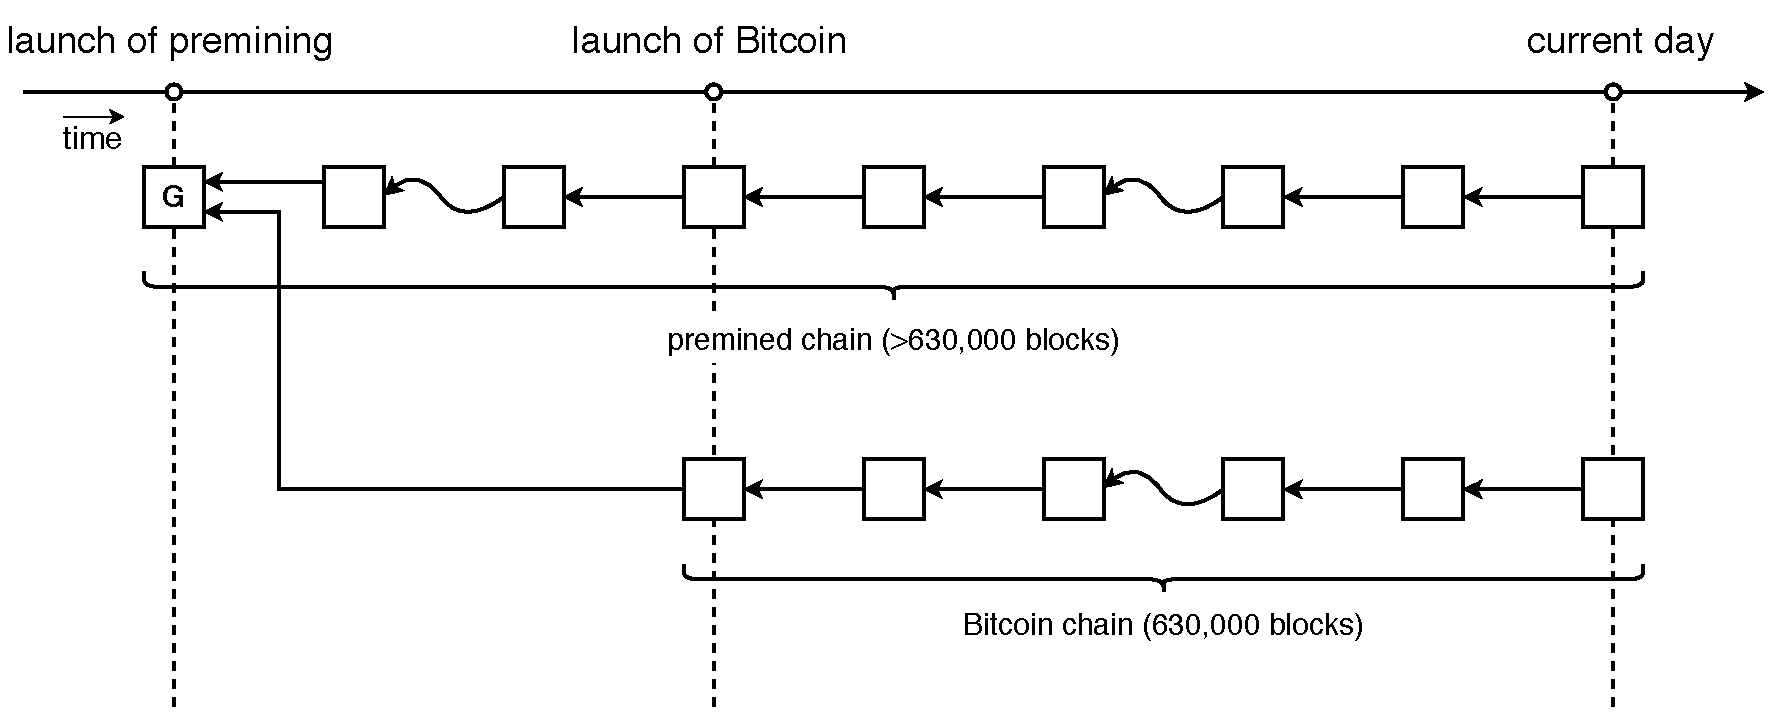
\includegraphics[width=12cm]{./images/premining_attack_bitcoin.pdf}

    \caption{ A premined chain started before the initiation of the public
    network. The older chain contains more blocks and proof-of-work.}

    \label{figure:premining_attack_bitcoin} \end{figure}



The NIPoPoW protocol takes into consideration the $genesis$ block of the
underlying blockchain. We remind that the first block of the chain is always
included in the NIPoPoW by construction. As we discuss in
Section~\ref{NIPoPoWs}, in the NIPoPoW protocol a proof is structurally correct
if two properties are satisfied:

\todo{Rewrite this with using the notation}

\begin{enumerate}[(a)]

\item The \emph{interlink} structure of all proof blocks is valid.

\item The first block of a proof for a chain $C$ is the first block $C$, the
    $genesis$ block.

\end{enumerate}

From property (b) of NIPoPoWs, we derive that the protocol is resilient to
premining because any chain that does not start from Bitcoin's $genesis$ block,
$gen_{B}$, results to a proof that also does not start from $gen_{B}$. Premined
chains start with blocks different than $gen_{B}$, hence NIPoPoW that describe
premined chains are invalid by definition.

\subsubsection{An attack} Previous implementation does require the existence of
underlying chain's $genesis$, exposing the verifier to premining attacks. Such
an attack can be launched by an adversary that mines new blocks on a chain $C'$
which is prior to the Bitcoin chain $C$ as displayed in
\begin{figure}[hbt] \centering

    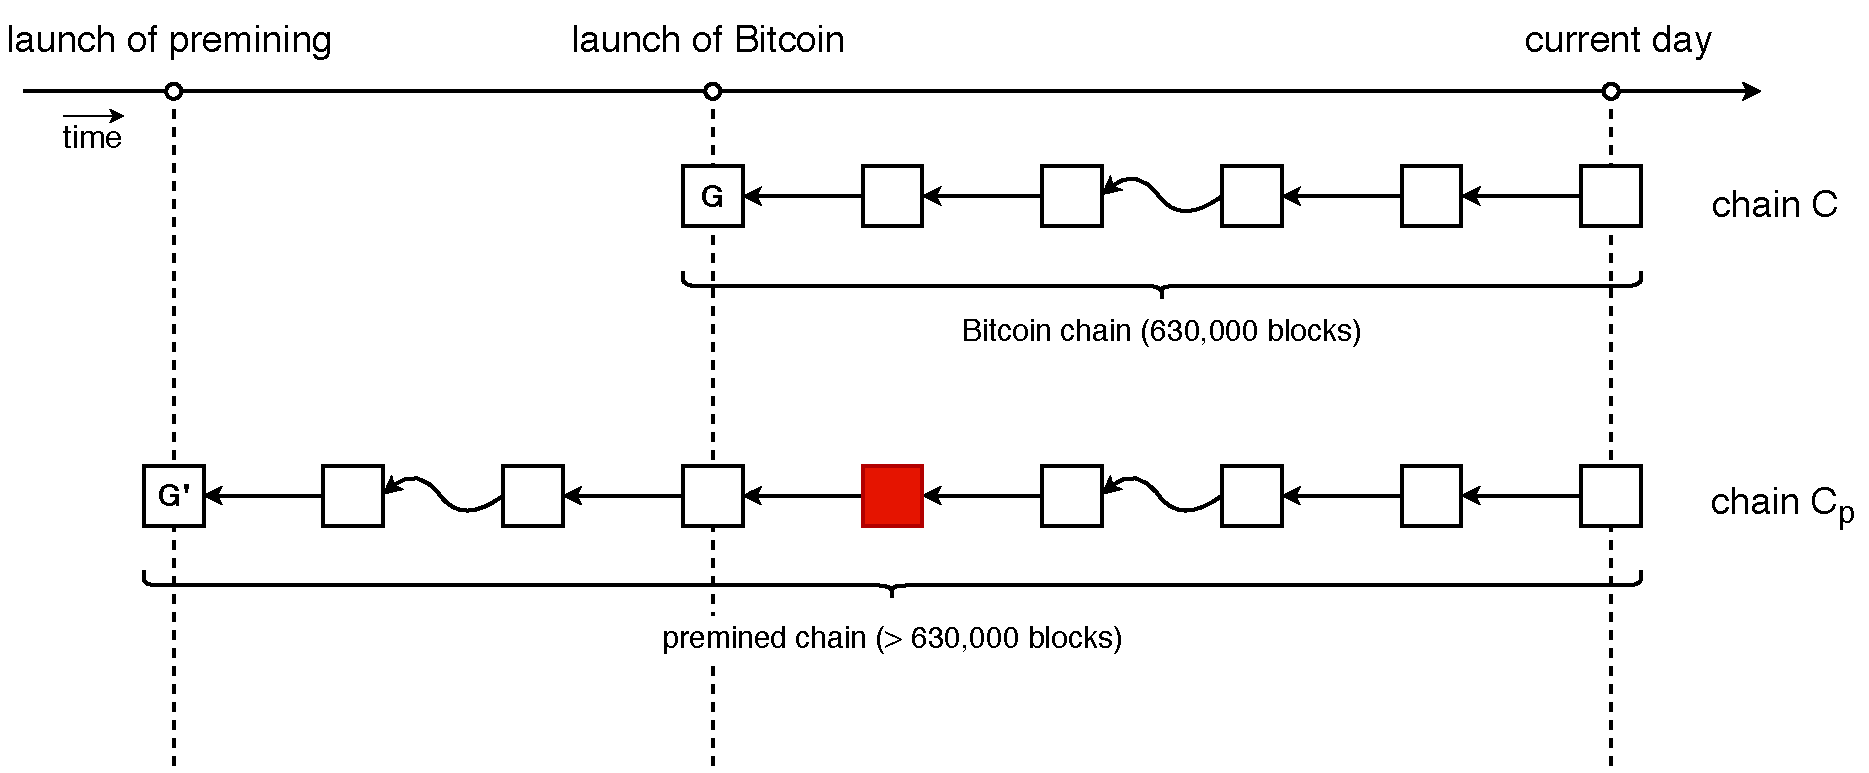
\includegraphics[width=12cm]{./images/premining_attack_nipopow.pdf}

    \caption{ A premined chain started before Bitcoin. The older chain contains
    more blocks.}

    \label{figure:premining_attack_nipopow} \end{figure}
 Proofs for events in $C'$ cannot
be contested by an honest party, since chain $C'$ includes more proof-of-work
than $C$ and thus NIPoPoWs with higher score can be generated.
Figure~\ref{figure:premining_attack_nipopow}.

\subsubsection{Mitigation}

We can mitigate this vulnerability by initializing the smart contract with the
$genesis$ block of the underlying blockchain (in our case, Bitcoin) persisting
$genesis$ in storage. For every phase, we add an assertion that the first block
of the proof must be equal to $genesis$. The needed changes are shown in
Algorithms~\ref{algo:avoid_premining_ctor}, ~\ref{algo:avoid_premining_submit}
and~\ref{algo:avoid_premining_contest}.

These operations do not increase the cost of the operations considerable
because the extra data saved in storage is constant and small in size (32
bytes).

\begin{algorithm}[H]

    \caption{\label{alg:avoid-premining}The \textsf{NIPoPoW} client mitigation
    to premining attack}
    \begin{algorithmic}[1]

    \Contract{crosschain}
    \State $\textsf{events} \gets \bot$; $\genesis \gets \bot$
    \State $\textsf{DAG} \gets \bot$; $\textsf{ancestors} \gets \bot$
    \Function{\sf initialize}{$\genesis_{remote}$}
        \State $\genesis$ $\gets \genesis_{remote}$
        \Comment{initialize with the genesis of the underlying chain}
    \EndFunction
    \Function{\sf submit}{$\pis$, $e$}
        \State \textsf{require}($\pis$[0] = $\genesis$)
        \Comment{assert correct genesis}
        \State \textsf{require}($\textsf{events$[e]$} = \bot$)
        \State \textsf{require}($\textsf{valid-interlinks}(\pi)$)
        \State \textsf{events$[e].\pi$} $\gets$ $\pis$
        \State \textsf{DAG} $\gets$ \textsf{DAG} $\cup$ $\pi$
        \State \textsf{ancestors} $\gets$ \textsf{find-ancestors(DAG, $\pi$[-1])}
        \State \textsf{require}(\textsf{evaluate-predicate}(\textsf{ancestors}, e))
        \State \textsf{ancestors} $=$ $\bot$
        \EndFunction
    \Function{\sf contest}{$\pic$, $e$}
        \State \textsf{require}($\pic$[0] = $\genesis$)
        \Comment{assert correct genesis}
        \State \textsf{require}(\textsf{events}$[e]$ $\ne$ $\bot$)
        \State \textsf{require}(\textsf{valid-interlinks}($\pic$))
        \State $lca$ = \textsf{find-lca}($\textsf{events}[e].\pi$, $\pic$)
        \State \textsf{require}($\pic$ $\geq_m$ $\textsf{events}[e].\pi$)
        \State \textsf{DAG} $\gets$ \textsf{DAG} $\cup$ $\pic$
        \State \textsf{ancestors} $\gets$
        \textsf{find-ancestors}($\textsf{DAG}$, $\textsf{events}[e].\pi$[-1])
        \State \textsf{require}($\neg$\textsf{evaluate-predicate}(\textsf{ancestors}, $e$))
        \State \textsf{ancestors} $=$ $\bot$
        \State \textsf{events$[e]$} $\gets$ $\bot$
    \EndFunction
    \EndContract
    \vskip8pt
    \end{algorithmic}
\end{algorithm}



\section{Storage Elimination}

A series of keen observations, the application of gas-efficient practices and
the utilization of modern Solidity features led us to the design of a new
verifier architecture. As mentioned above, the bottleneck we had to eliminate
was the extensive usage of storage. our implementation is bases on a new
architecture that allow us to discard all expensive store operations and
utilize memory instead, which led to massive decrease of gas consumption. We
call this technique \emph{hash-and-resubmit}.

In this section, we present the performance difference in gas consumption
between storage and memory utilization. Then, we show how a gas-efficient,
superlight Bitcoin client can be implemented in Solidity without persisting
proofs, utilizing our novel technique.

We will use extend our annotation with the content of
Table~\ref{table:notation_verifier}.

\begin{table}[H]
\begin{tabular}{ll}
\hline
\multicolumn{1}{|c|}{Symbol} & \multicolumn{1}{c|}{Description} \\ \hline
$\es$      & The entity initiating submit-phase \\
$\ec$      & The entity initiating contest-phase \\
$\pis$    & The proof submitted by $\es$ \\
$\pisa$   & A copy of $\pi_{subm}$ submitted by $\ec$ \\
$\pic$    & The contesting proof submitted by $\ec$ \\

\end{tabular}
\centering
\caption{Notation}
\label{table:notation_verifier}
\end{table}


\subsection{Storage vs Memory}

We will first demonstrate the difference in gas usage between storage and
memory for a smart contract in Solidity. Suppose we have the following simple
contract:

\lstinputlisting[style=customc, captionpos=b, label={listing:storage_memory},
caption={Solidity test for storage and memory}]{code/StorageVsMemory.sol}
\todo{Highlight code}

Function \texttt{withStorage()} populates an array saved in storage and
function \texttt{withMemory()} populates an array saved in memory. We
initialize the sizes of the arrays by passing the variable \texttt{size} to the
contract constructor. We run this piece of code for \texttt{size} from 1 to
100. The results are displayed at Figure~\ref{figure:memory_vs_storage}. For
\texttt{size} = 100, the gas expended is 53,574 gas units using memory and
2,569,848 using storage which is almost 50 times more expensive. This code was
compiled with Solidity version 0.6.6 with optimizations enabled\footnote{This
version of Solidity compiler, which was the latest at the time this paper was
published, did not optimize-out any of the variables.}. The EVM we used  was
Ganache at the latest Constantinople(ref) fork. It is obvious that if there is
the option to use memory instead of storage in the design of smart contracts,
the choice of memory greatly benefits the users.

\begin{figure}
\centering
\begin{tikzpicture}
    \begin{axis}[
        y tick label style={/pgf/number format/.cd,%
          set thousands separator={,},
          fixed},
        legend pos=north west,
        scaled y ticks = false,
        grid=major,
        xlabel={Array size},
        ylabel={Gas consumption}]
    \addplot table [mark=none, col sep=comma] {data/storage.csv};
    \addplot table [mark=none, col sep=comma] {data/memory.csv};
    \legend{$storage$,$memory$};
\end{axis}
\end{tikzpicture}
\caption{Gas consumption for memory and storage}
\label{figure:memory_vs_storage}
\end{figure}


\subsection{Refining Ancestors}

We observed that in the code of the verifier the existence of
\texttt{ancestors}$_s$ structure is redundant. The lifetime of the structure is
limited within the last lines of each phase, and serves the role of temporary
storing the result of \texttt{evaluatePredicate}, and then it is deleted. The
same functionality can be achieved if the \texttt{ancestor}$_s$ is saved in
memory rather than in the storage of the contract. The changes needed in order
to convert \texttt{ancestors}$_s$ into a memory structure is displayed in
Algorithm~\ref{algorithm:ancestors_in_memory}.

\begin{algorithm}[H]
    \caption{Usage of memory ancestors}
    \label{algorithm:ancestors_in_memory}
    \KwIn{\texttt{Proof} $\pi$, \texttt{Predicate} $predicate$}
    \KwData{
        \texttt{Block} $genesis_{s}$,
        \texttt{Proof} $\pi_{s}$,
        \texttt{hashmap} $DAG_{s}$,
        \texttt{bool} $predicateExists_{s}$
    }
    require $\pi[0]$ = $genesis_{s}$ \\
    require($predicateExists_{s}$ $=$ $false$) \\
    require($validInterlink(\pi$))\\
    $DAG_{s}$ $\leftarrow$ $DAG_{s}$ $\cup$ $\pi$\\
    $\pi_{s}$ $\leftarrow$ $\pi$\\
    \colorbox{green}{$ancestors_{m}$ $\leftarrow$ $findAncestors(DAG_{s}$)} \\
    \colorbox{green}{$predicateExists_{s}$ $\leftarrow$
    $evaluatePredicate(ancestors_{m}$, $predicate$)} \\
\end{algorithm}


The elimination of storage structures results to better performance of the
contract. In Table~\ref{table:old_gas_usage_no_ans} we show how such a subtle
refinement can lead to a sizable performance gain.

\begin{table}[H]
    \centering
    \begin{tabular}{|l|r|r|r|}
    \hline
    \multicolumn{4}{|c|}{\textbf{Submit Phase}}          \\ \hline
    \multicolumn{1}{|c|}{\textbf{Function}} &
      \multicolumn{1}{c|}{\textbf{\begin{tabular}[c]{@{}c@{}}Storage\end{tabular}}} &
      \multicolumn{1}{c|}{\textbf{\begin{tabular}[c]{@{}c@{}}Memory\end{tabular}}} &
      \multicolumn{1}{c|}{\textbf{\begin{tabular}[c]{@{}c@{}}Performance \\ Gain\end{tabular}}} \\ \hline
    find ancestors     & 4,995,289  & 3,776,205 & 24.40\%  \\ \hline
    evaluate predicate & 306,433    & 191,489   & 60.00\%  \\ \hline
    delete ancestors   & 45,137     & 0         & 100.00\% \\ \hline
    \textbf{Sum}       & 10,025,780 & 8,913,990 & \textbf{0.11\%}   \\ \hline
    \end{tabular}
    \quad
    \begin{tabular}{|l|r|r|r|}
    \hline
    \multicolumn{4}{|c|}{\textbf{Contest Phase}}          \\ \hline
    \multicolumn{1}{|c|}{\textbf{Function}} &
      \multicolumn{1}{c|}{\textbf{\begin{tabular}[c]{@{}c@{}}Storage\end{tabular}}} &
      \multicolumn{1}{c|}{\textbf{\begin{tabular}[c]{@{}c@{}}Memory\end{tabular}}} &
      \multicolumn{1}{c|}{\textbf{\begin{tabular}[c]{@{}c@{}}Performance \\ Gain\end{tabular}}} \\ \hline
    find ancestors     & 5,584,173  & 4,162,519 & 25.50\%  \\ \hline
    evaluate predicate & 390,307    & 153,209   & 60.00\%  \\ \hline
    delete ancestors   & 57,023     & 0         & 100.00\% \\ \hline
    \textbf{Sum}       & 10,361,330 & 8,878,148 & \textbf{0.14\%}   \\ \hline
    \end{tabular}

\caption{Gas consumption degradation with memory for ancestors}
\label{table:old_gas_usage_no_ans}
\end{table}


\subsection{Refining Predicate}

\todo{predicate is not needed in contest phase}

\subsection{Hash and resubmit}

In previous work storage was needed to persist submitted proofs and perform
contests. In this subsection we show out novel approach to securely verify
proofs without utilizing the persistent storage. We name this technique
\emph{hash-and-resubmit}.

The rationale is to demand from $E_{cont}$ to provide two proofs to the
contract during contest phase: (a) $\pi_{exist}$, which is a copy of the
originally submitted proof $\pi_{orig}$, and (b) $\pi_{cont}$, which is the
contesting proof. The challenge here, is twofold:

\begin{enumerate}

    \item Availability: $E_{cont}$ must be able to retrieve a valid copy of $\pi_{orig}$,
        $\pi_{exist}$ without the need of accessing on-chain data.

    \item Reliability: We must prevent $E_{cont}$ from dispatching
        $\tilde\pi_{exist}$ which differs from $\pi_{orig}$.

\end{enumerate}

Hash-and-resubmit is utilized in two phases in order to face this challenge.
The "resubmit" aspect addresses availability, and the "hash" aspect addresses
reliability.

\paragraph{Addressing Availability}

During submit-phase, $E_{subm}$ makes a call to the function
\texttt{submitEventProof}. This transaction, which consists of (a) the function
call and (b) the corresponding data, is added to a block by a miner. As a
blockchain transaction, the data of the function call are public to the
network. Due to blockchain's transparency, $E_{cont}$ can retrieve
$\pi_{orig}$ without the need of accessing contract data. This data space is
called \emph{calldata}, and we make use of it to fetch $\pi_{exist}$, which is
an exact copy of $\pi_{orig}$, originally submitted by $E_{subm}$. Note that
this process is done off-chain. $E_{cont}$ does not have to interact with the
client.

\paragraph{Addressing Reliability}

We prevent an adversary from altering $\pi_{exist}$ by storing the hash of
$\pi_{orig}$ in contract's state during submit phase and then verifying that
$\pi_{exist}$ has the same hash. The operation of hashing the proof and storing
the digest is cheap as shown in figure~\ref{figure:hash_proof_gas}. We
calculate the digest by invoking the pre-compiled \texttt{sha256} hash function
of Solidity:

\[\texttt{digest = sha256(abi.encodePacked(proof))}\] The size of the digest of
a hash is 32 bytes. To persist such a small value in contract's memory only
adds a constant, negligible cost overhead to our implementation. This low-cost
technique allows us to provide vastly improved performance compared to the
previous work as we will show in the following subsections.

\begin{figure}
\centering
\begin{tikzpicture}
    \begin{axis}[
        y tick label style={/pgf/number format/.cd,%
          set thousands separator={,},
          fixed},
        legend pos=north west,
        scaled y ticks = false,
        grid=major,
        xlabel={Proof size},
        ylabel={Gas consumption}]
    \addplot table [col sep=comma] {data/hash_proof_gas.csv};
    \legend{sha256 gas cost};
\end{axis}
\end{tikzpicture}
\caption{Gas consumption for hashing proofs and storing digest}
\label{figure:hash_proof_gas}
\end{figure}



\subsection{Removing DAG and ancestors}

In this subsection we show how these two structures can be discarded from the
client entirely. As shown in table~\ref{table:old_gas_usage}, the most
demanding operation is the creation and population of DAG and ancestors. We
show how ancestors structure can be improved, but the performance gain from
this change still fails to deliver a client that is practical in a real
setting.

Now that we have achieved to freely retrieve $\pi_{exist}$, we can start
sketching methodologies that benefit from this schema but another challenge we
had to face is that the protocol of NIPoPoWs dependents on DAG which is a
hashmap data structure. While such data structures are very efficient and
useful data structures, in Solidity, hashmaps can only be contained in storage,
which is unpromising for an efficient client design. Having that in mind, we
created a schema that does not require the DAG, ancestors or any other
complementary structures.


\subsubsection{Using subset}

Our first realization was that instead of creating a DAG of $\pi_{exist}$ and
$\pi_{cont}$, we can rather require

\[ \pi_{exist}\{:\textrm{LCA}\} \subseteq \pi_{cont}\{:\textrm{LCA}\} \]
This way, we avoid the burden of maintaining auxiliary structures DAG and
ancestors on-chain. The implementation of \texttt{subset} is displayed in
listing~\ref{listing:subset}. The complexity of the function is \[
\mathcal{O}(|\pi_{exist}\{:LCA\}| + |\pi_{cont}\{:LCA\}]|) \]

\lstinputlisting[style=customc, captionpos=b, label={listing:subset},
caption={Implementation of subset}]{code/Subset.sol}

\begin{figure}[ht]
\begin{subfigure}{.5\textwidth}
  \centering
  % include first image
  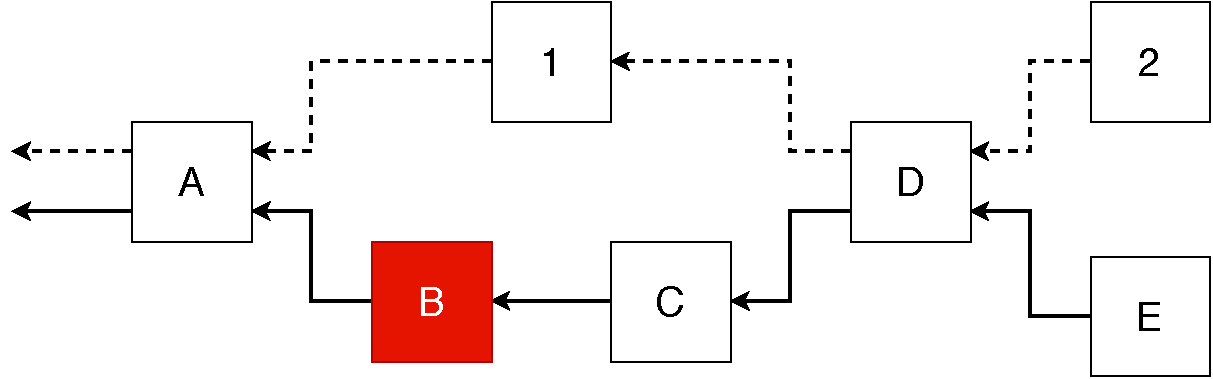
\includegraphics[width=6cm]{../images/Subset_1.pdf}
  \caption{Valid $\pi_{cont}$ before using subset}
  \label{figure:DAG_usage}
\end{subfigure}
\begin{subfigure}{.5\textwidth}
  \centering
  % include second image
  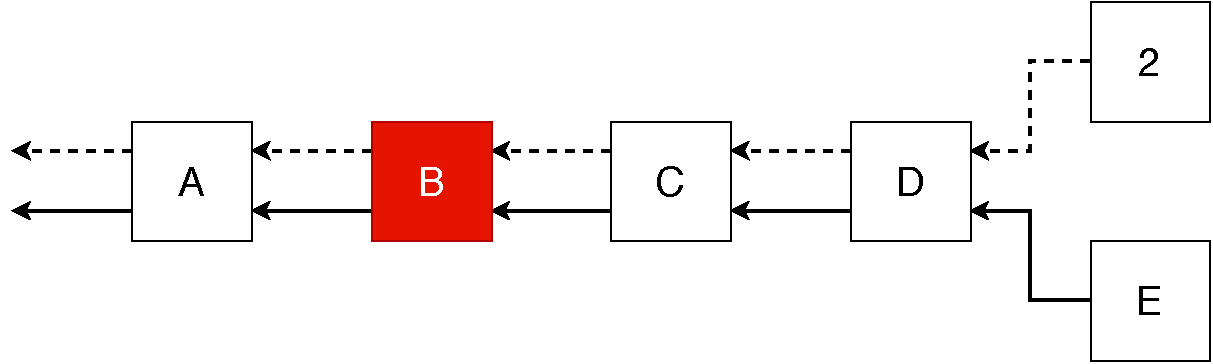
\includegraphics[width=6cm]{../images/Subset_2.pdf}
  \caption{Valid $\pi_{cont}$ after using subset}
  \label{figure:DAG_usage}
\end{subfigure}
\caption{Blocks connected with solid lines indicate $\pi_{exist}$ and blocks
connected with dashed lines indicate $\pi_{cont}$}
\label{fig:fig}
\end{figure}


The gas consumption difference between $subset$ and $DAG+ancestors$ is
displayed at figure~\ref{figure:DAG_vs_subset}. $Subset$ solution is
approximately 2.7 times more efficient.

\begin{figure}
\centering
\begin{tikzpicture}
    \begin{axis}[
        y tick label style={/pgf/number format/.cd,%
          set thousands separator={,},
          fixed},
        legend pos=north west,
        scaled y ticks = false,
        grid=major,
        xlabel={Proof size},
        ylabel={Gas consumption x 1.000}]
    \addplot table [col sep=comma] {data/DAG_ancestors.csv};
    \addplot table [col sep=comma] {data/subset.csv};
    \legend{$DAG+ancestors$,$Subset$};
\end{axis}
\end{tikzpicture}
\caption{Gas consumption for DAG+ancestors and subset}
\label{figure:DAG_vs_subset}
\end{figure}


\subsubsection{Subset complexity and limitations}

Requiring $\pi_{exist}$ to be a subset of $\pi_{cont}$ greatly reduces gas, but
the complexity of the $subset$ algorithm is high since both proofs have to be
iterated from $Gen$ until $lca_e$ and $lca_c$, respectively. Generally, we
expect from an adversary to provide a proof of a chain that is a fork of the
honest chain at some point relatively close to the tip. This is due to the fact
that the ability of an adversary to sustain a fork chain exponentially weakens
as the honest chain progresses. This means that the length of $\pi$, $|\pi|$ is
expected to be considerably close to $|\pi[:lca]|$, and thus the complexity of
\texttt{subset()} effectively becomes $\mathcal{O}(2|\pi|)$.

In realistic cases, where LCA lies around index 250 of the proof, the gas cost
of \texttt{subset()} is approximately 20,000,000 gas units, which makes it
inapplicable for real blockchains since it exceeds the block gas limit of the
Ethereum blockchain by far.

\subsubsection{Position of block of interest}

By analyzing the benefits and trade-offs of $subset$, we concluded that there
is a more efficient way to treat storage elimination. In general, the concept
of $subset$ facilitated the case in which the block of interest belongs in the
sub-proof $\pi_{exist}[:lca_{e}]$. But in this case, both $\pi_{exist}$ and
$\pi_{cont}$ contain the block of interest at some index, as can be seen in
figure~\ref{figure:after_subset}. Consequently, $\pi_{cont}$ cannot contradict
the existence of the block of interest and the predicate is evaluated $true$
for both proofs. This means that if (a) $\pi_{exist}$ is structurally correct
and (b) the block of interest is in $\pi_{exist}[:lca_{e}]$, then we can safely
conclude that contesting with $\pi_{cont}$ is redundant. Therefore,
$E_{contest}$ can simply send $\pi_{cont}$[lca:] to the verifier. The
truncation of $\pi_{cont}$ to $\pi_{cont}[lca_{c}:]$ can be easily addressed
from $E_{cont}$, since $\pi_{exist}$ is accessible from the contract's
calldata and both proofs can be iterated off-chain.

\newcommand*{\exist}{$\pi_{exist}$}
\newcommand*{\cont}{$\pi_{cont}^{tr}$}

\subsubsection{Disjoint proofs}

We will refer to the truncated contesting proof as $\pi_{cont}^{tr}$ and to
$lca_{e}$ simply as $lca$. For the aforementioned, the following statements are
true:

\begin{enumerate}[(a)]
    \item  $\pi_{exist}[0]$ = $genesis$
    \item  $\pi_{exist}[lca]$ = $\pi_{cont}^{tr}[0]$
\end{enumerate}

The requirement that needs to be satisfied is
\[\pi_{exist}\{lca+1:\} \cap \pi_{cont}^{tr}\{1:\} = \emptyset \]

The implementation of this operation is shown in
listing~\ref{listing:disjoint}.

\lstinputlisting[style=customc, captionpos=b, label={listing:disjoint},
caption={Implementation for disjoint proofs}]{code/Disjoint.sol}

The complexity of \texttt{disjoint()} is
\[ \mathcal{O}(|\pi_{exist}[lca_{e}:]| \times
|\pi_{cont}^{tr}|) \]

\section{Fixing vulnerabilities and restricting gas usage}

% \begin{itemize}
%
%     \item
%         This is not vulnerable to DOS attacks
%
% \end{itemize}
